\documentclass[]{article}

\usepackage{amsmath}
\usepackage{amssymb}
\usepackage{graphicx}
\usepackage{float}
\usepackage{multicol}
\usepackage{fancyhdr}
\fancyhead[L, CO] {}
\fancyhead[C, CO] {AppElm - Résumé 2022}
\fancyhead[R, CO] {}
\usepackage[margin=1.5cm,landscape]{geometry}
\pagestyle{fancy}
\usepackage{mathtools} % for '\splitdfrac' macro
\usepackage[dvipsnames]{xcolor}
\usepackage{subfiles}
\usepackage{mdframed}
\usepackage{siunitx}
\usepackage{amsmath}
\usepackage{amssymb}
\usepackage{physics}
\usepackage{mathrsfs}
\usepackage{enumitem}
\setlist[itemize]{nosep, itemsep=0pt, leftmargin=0.5cm}
\setlist[enumerate]{nosep, itemsep=0pt, leftmargin=0.5cm}
\DeclareMathOperator{\Div}{div}
\DeclareMathOperator{\Rot}{rot}


\begin{document}
\begin{multicols}{3}
\subfile{lf}
\end{multicols}
\begin{multicols}{2}
\begin{center}
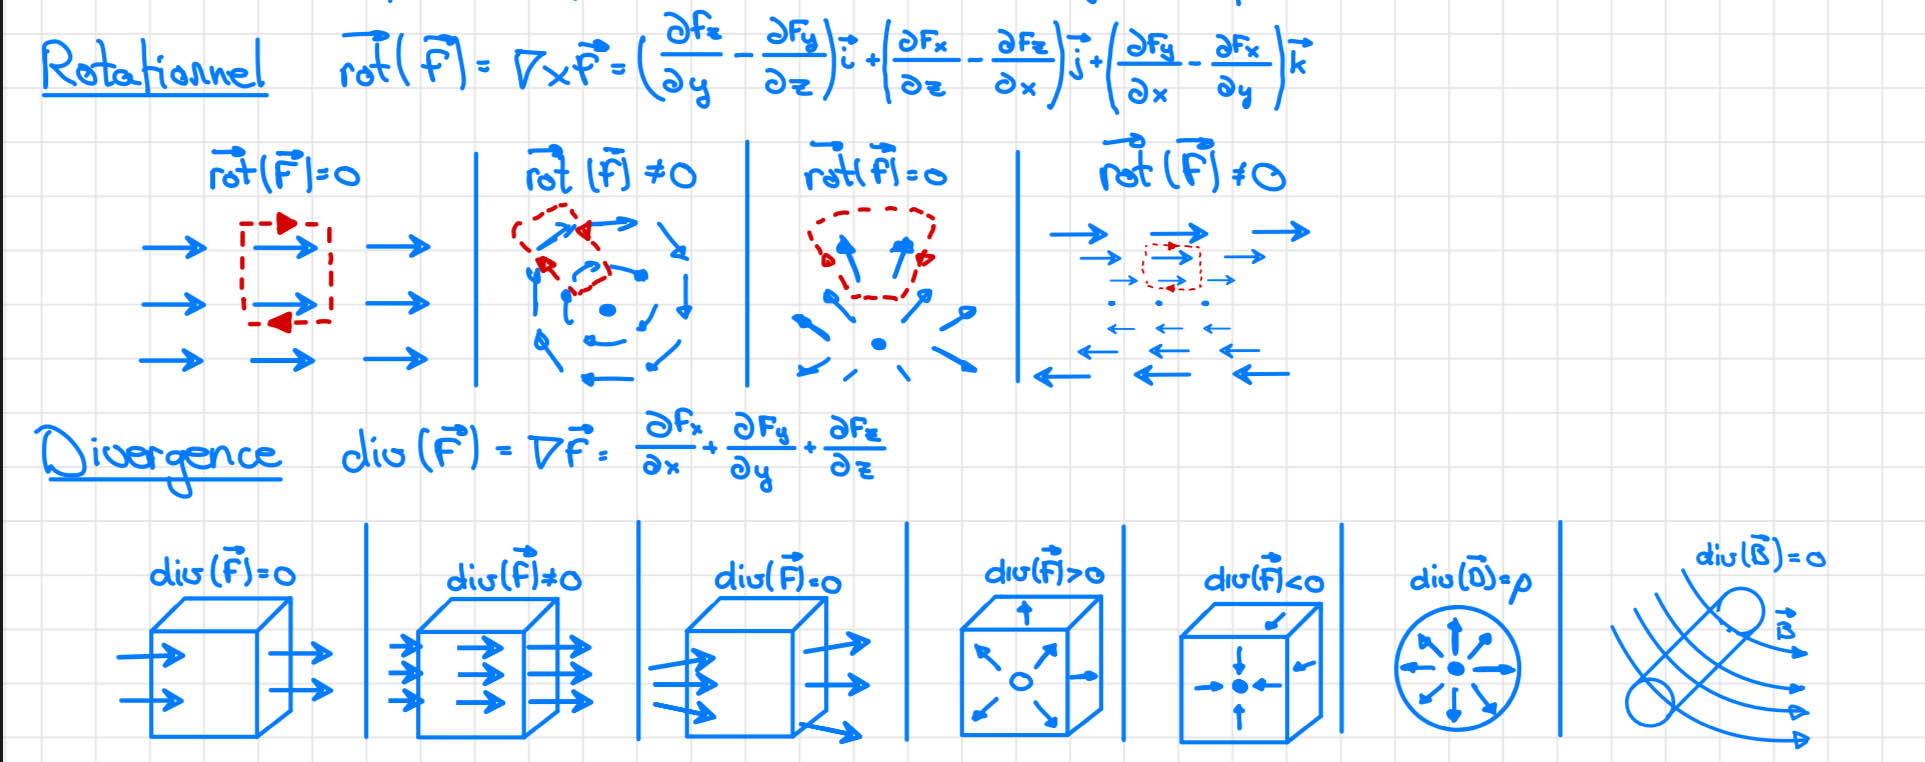
\includegraphics[width=10cm]{MicrosoftTeams-image.png}
\end{center}
Rotationel négatif lorsqu'il tourne dans le sens des aiguilles d'une montre.
\end{multicols}
\pagebreak
\begin{multicols}{3}
\subfile{hf}
\end{multicols}
\end{document}